\section{Graph clustering and community recovery}
\label{sec:community-detection}


\begin{figure}
\begin{center}
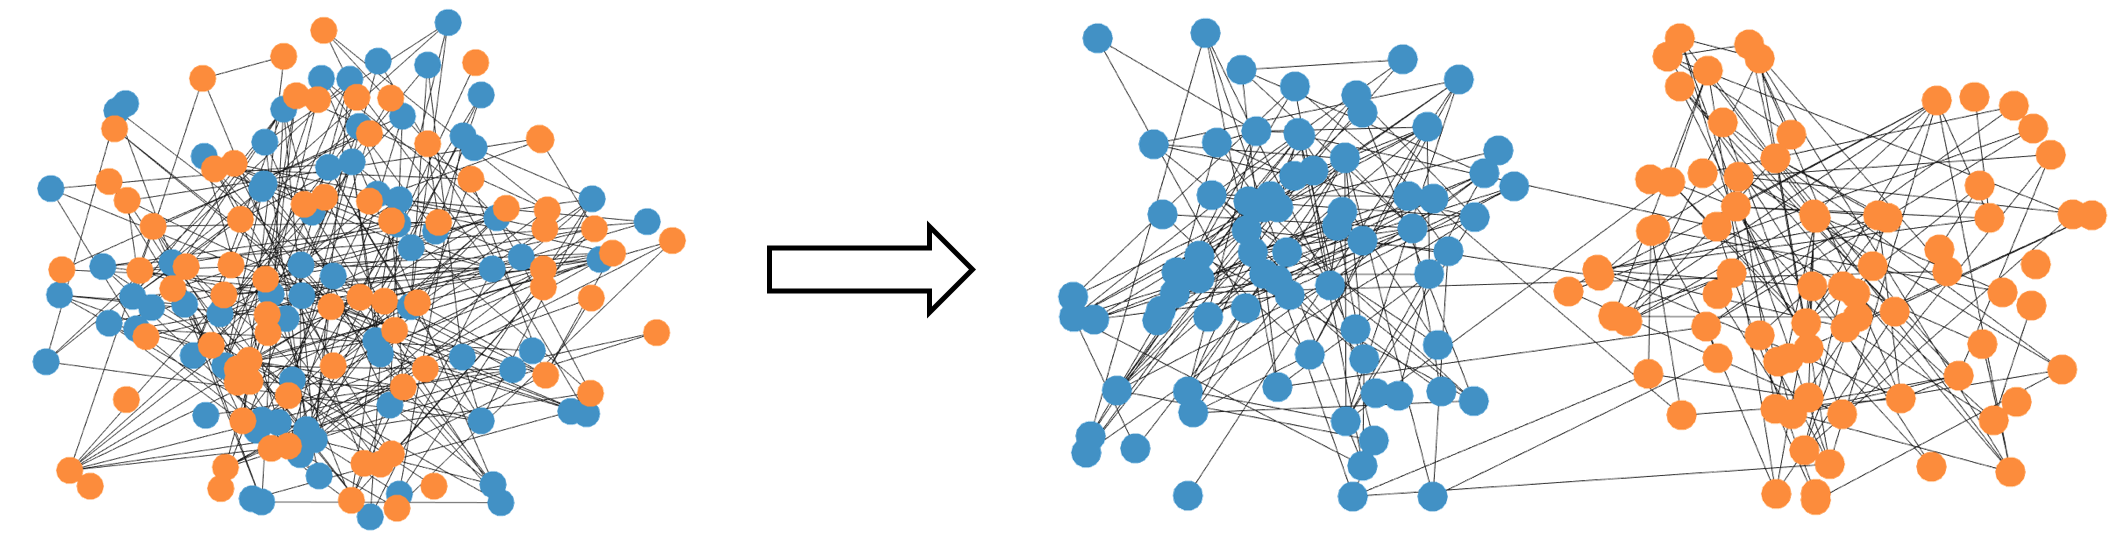
\includegraphics[width=0.85\textwidth]{figures/SBM_illustrate.png}
\end{center}
\caption{Illustration of graph clustering and community recovery, where one wishes to cluster all nodes into two communities based on the edges in the graph.} \label{fig:community}
\end{figure}


Next, we move on to a central problem that permeates data science applications: clustering. An important formulation that falls under this category is graph clustering or community recovery, which aims to cluster individuals into different communities based on  pairwise measurements of their relationships, each of which reveals information about whether or not two individuals belong to the same community \citep{abbe2017community}; see Figure~\ref{fig:community} for an illustration. There has been a recent explosion of interest in this problem, due to its wide applicability in, say, social network analysis \citep{azaouzi2019community}, image segmentation \citep{browet2011community}, shape mapping in computer vision \citep{huang2013consistent}, haplotype phasing in genome sequencing \citep{chen2016community}, to name just a few.
This section explores the capability of spectral methods in application to graph clustering;
 we will revisit the clustering problem again in Section~\ref{sec:Gaussian-mixture} for another common formulation.



\subsection{Problem formulation and assumptions}
\label{sec:setup-community-detection}


In this section, we formulate the graph clustering problem via the well-renowned {\em stochastic block model} (SBM) introduced in \citet{holland1983stochastic}---an idealized generative model that commonly serves as a  theoretical benchmark for evaluating community recovery algorithms.




Consider an undirected graph $\mathcal{G}=(\mathcal{V},\mathcal{E})$ that comprises $n$ vertices, where $\mathcal{V}$ and   $\mathcal{E}$ denote the vertex set and the edge set of $\mathcal{G}$, respectively.  The $n$ vertices, labelled by $1,\cdots, n$,
exhibit  community structures and can be grouped into two non-overlapping communities of {\em equal} sizes. Here and throughout,  $n$ is assumed to be an even number, so that each community contains exactly $n/2$ vertices.
To encode the community memberships, we assign $n$ binary-valued variables $x_i^{\star} \in \{1,-1\}$ ($1\leq i \leq n$) to the  vertices in a way that
%
\begin{align*}
	x_i^{\star} = \begin{cases} 1, \qquad & \text{if vertex } i \text{ belongs to the 1st community}, \\
				   -1, \quad  & \text{otherwise}. \end{cases}
\end{align*}
%




The SBM assumes that the set $\mathcal{E}$ of (undirected) edges  is generated randomly based on the community memberships of the incident vertices. To be precise, each pair $(i,j)$ of vertices  is  connected by an edge independently with probability $p$ (resp.~$q$) if $i$ and $j$ belong to the same community (resp.~different communities). The resultant connectivity pattern is represented by an adjacency matrix
$\bm{A}=[A_{i,j}]_{1\leq i,j\leq n}\in \{0,1\}^{n\times n}$, such that for each pair $(i,j)$,
%
\begin{align}
	A_{i,j} = \begin{cases} 1, \qquad & \text{if }(i,j)\in \mathcal{E}, \\ 0, & \text{otherwise}.   \end{cases}
\end{align}
%
By convention, we take the diagonal entries to be $A_{i,i}=0$ for all $1\leq i\leq n$. As a remark, the matrix $\bm{A}$ is symmetric since $\mathcal{G}$ is an undirected graph,  with upper triangular elements being realizations of independent Bernoulli random variables with mean either $p$ (if two nodes are in the same community) or $q$ (otherwise).  In addition, it is assumed throughout that $p>q>0$, implying that there are in expectation more within-community edges than across-community edges.

Based on the adjacency matrix $\bm{A}$ generated by the SBM,
the goal is to identify the latent community memberships of the vertices. To phrase it in mathematical terms,
the aim is to reconstruct the vector  $\bm{x}^{\star}=[x_i^{\star}]_{1\leq i\leq n}\in \{1,-1\}^n$ modulo the global sign,
namely, recovering either $\bm{x}^{\star}$ or $-\bm{x}^{\star}$.
This is all one can hope for, as there is
absolutely no basis to distinguish the names of two groups.
%$\bm{x}^{\star}$ from $-\bm{x}^{\star}$ given merely the edge information.




\subsection{Algorithm: spectral clustering}
\label{sec:algorithm-community-detection}

Now we describe a spectral method.
To simplify presentation, it is assumed without loss of generality that: $x_i^{\star}=1$ for any $1\leq i\leq n/2$, and $x_i^{\star}=-1$ for any $i > n/2$.


A starting point for the algorithm design is to examine the mean of the adjacency matrix,  given as follows
%
\begin{align*}
	 \mathbb{E}[\bm{A}]  	=
	\left[\begin{array}{cc}
		p\,\bm{1}_{n/2}\bm{1}^{\top}_{n/2} & q\,\bm{1}_{n/2}\bm{1}^{\top}_{n/2}\\
		q\,\bm{1}_{n/2}\bm{1}^{\top}_{n/2} & p\,\bm{1}_{n/2}\bm{1}^{\top}_{n/2}
	\end{array}\right] -   p \bm{I}.
\end{align*}
%
As revealed by the above calculation,   the  matrix constructed below
%
\begin{align}
	\bm{M} = \bm{A} -\frac{p+q}{2} \bm{1}_n\bm{1}^{\top}_n  + p\bm{I}
	\label{eq:M-data-matrix-SBM}
\end{align}
%
exhibits an approximate rank-1 structure, in the sense that its mean
%
\begin{align} \label{eq:M-data-matrix-expectation-SBM}
	\bm{M}^{\star} \coloneqq \mathbb{E}[\bm{M}] =
	\frac{p-q}{2}\left[\begin{array}{c}
		\bm{1}_{n/2}\\
		-\bm{1}_{n/2}
	\end{array}  \right] \left[\begin{array}{cc}
\bm{1}^{\top}_{n/2} & -\bm{1}^{\top}_{n/2}\end{array}\right]
\end{align}
%
is a rank-1 matrix.  The leading eigenvalue of $\bm{M}^{\star}$ and its associated eigenvector are given respectively by
%
\begin{align}
	\lambda^{\star}\coloneqq\frac{(p-q)n}{2},  
	\quad \text{and} \quad
	\bm{u}^{\star}  \coloneqq \frac{1}{\sqrt{n}}
	\left[\begin{array}{c}
		\bm{1}_{n/2}\\
		-\bm{1}_{n/2}
	\end{array}\right].
	\label{eq:leading-evalue-evector-M-SBM}
\end{align}
%
Crucially, the eigenvector  $\bm{u}^{\star}$ encapsulates the precise community structure we seek to recover: all positive entries of $\bm{u}^{\star}$ correspond to vertices from one community, while the remaining ones form another community.



Inspired by the above calculation, a candidate spectral clustering algorithm consists of eigendecomposition followed by entrywise rounding:
%
\begin{itemize}
	\item[1.] Compute the leading eigenvector $\bm{u}$ of  $\bm{M}$ (constructed in \eqref{eq:M-data-matrix-SBM});
	\item[2.] Compute the estimate $\bm{x}=[x_i]_{1\leq i\leq n}$  such that for any $1\leq i\leq n$,
	%
	\begin{align}
		  x_{i}= \mathsf{sgn}(u_i)  =
		  \begin{cases}
1,\quad & \text{if }u_{i}>0,\\
-1, \quad & \text{if }u_i \leq 0.
\end{cases}
	\end{align}
\end{itemize}
%
% Here, for any $z\in \mathbb{R}$, the sign function obeys $\mathsf{sgn}(z)=1$ if $z>0$ and $\mathsf{sgn}(z)=-1$ otherwise. 
In words, the community memberships are estimated in accordance with the signs of the entries of the leading eigenvector of $\bm{M}$, namely, the entries with the same signs are declared to come from the same cluster.

%which has two non-vanishing eigenvalues and their associated eigenvectors
%$$
%  	\lambda_1^* = \frac{(p+q)n}{2},~\lambda_2^* = \frac{(p-q)/n}{2},  \mbox{ and }  \bu_1^* = \frac{1}{\sqrt{n}}\mathbf{1}, ~ 	\bu_2^*=\frac{1}{\sqrt{n}}\left[\begin{array}{c}
%  		\bm{1}_{n/2}\\
%  		-\bm{1}_{n/2}
%  	\end{array}  \right ].
%$$
%Therefore, the second eigenvector reveals the true membership of the community.  We can work directly with the second eigenvector, but we here work with the first eigenvector by shifting the first component $\lambda_1^* \bu_1^*  (\bu_1^* )^T$  in the eigen-decomposition.  

\begin{remark}
	The above algorithm requires prior knowledge of the parameters $p$ and $q$ when constructing  $\bm{M}$. It is also feasible to develop a ``model-agnostic'' alternative by, for instance, looking at the second eigenvector of $\bm{A}$ (since the second eigenvector of $\mathbb{E}[\bm{A}]$ turns out to be precisely $\bm{u}^{\star}$), which does not rely on prior information about $p$ and $q$ at all; see, e.g., \citet{abbe2020entrywise} for details.  Here, we adopt the above model-dependent version primarily for convenience of exposition.  %To make the method feasible, we note that $ \mathbb{E} \sum_{i,j} A_{i, j} = n^{2}(p+q)/2 - n p$ and we can estimate $p+q$ by $2n^{-2} \sum_{i,j}A_{i,j}$ in the construction of $M$.
\end{remark}


\subsection{Performance guarantees: almost exact recovery}
\label{sec:theory-community-detection}

The spectral method enjoys appealing statistical guarantees for recovering the community structure of the SBM, which can be readily obtained by invoking the $\ell_2$ eigenvector perturbation theory.  To demonstrate this, we begin by developing an upper bound on the spectral norm of the perturbation matrix $\bm{E}\coloneqq \bm{M} - \bm{M}^{\star}$,
postponing the proof to Section~\ref{sec:proof-auxiliary-lemmas-community-detection}.
%
\begin{lemma} \label{lemma:E-spectral-norm-SBM}
	Consider the settings in Section~\ref{sec:setup-community-detection}, and suppose that $np\gtrsim \log n$. Then with probability at least $1-O(n^{-8})$, one has
	%
	\begin{align}
		\| \bm{E} \| \lesssim \sqrt{np} .
	\end{align}
\end{lemma}
%
This spectral norm bound, in conjunction with the Davis-Kahan sin$\bm{\Theta}$ theorem, leads to the following theoretical support for the spectral method introduced in Section~\ref{sec:algorithm-community-detection}.
%
\begin{theorem}
	\label{thm:community-detection-weak}
	Consider the setting in Section~\ref{sec:setup-community-detection}, and suppose that
	%
	\begin{align}
		p \gtrsim\frac{\log n}{n}, 
		\qquad\text{and}\qquad \sqrt{\frac{p}{n}} =o(p-q).
		\label{eq:assumption-p-q-SBM-L2}
	\end{align}
	With probability exceeding $1-O(n^{-8})$, the spectral method achieves
	%
	\begin{align*}
		\frac{1}{n}\sum_{i=1}^{n}\mathbbm1\big\{ x_{i} = x_{i}^{\star}\big\} = 1- o(1), 
		\quad \text{or} \quad
		\frac{1}{n}\sum_{i=1}^{n}\mathbbm1\big\{ x_{i} = - x_{i}^{\star}\big\} = 1- o(1) .
	\end{align*}
	%
\end{theorem}
%
It is noteworthy that the metric
%
\[
	\min \Bigg\{  \frac{1}{n}\sum_{i=1}^{n}\mathbbm1\big\{ x_{i} \neq x_{i}^{\star}\big\},\, \frac{1}{n}\sum_{i=1}^{n}\mathbbm1\big\{ x_{i} \neq - x_{i}^{\star}\big\} \Bigg\}
\]
%
can be understood as the mis-clustering rate.
In a nutshell, Theorem~\ref{thm:community-detection-weak} asserts that with the assistance of simple rounding (i.e., the $\mathsf{sgn}(\cdot)$ operation), the spectral method allows for {\em almost} exact community recovery---namely, correctly clustering all but a vanishing fraction of the vertices---assuming satisfaction of Condition~\eqref{eq:assumption-p-q-SBM-L2}.  Note that ``almost exact recovery'' is also referred to as ``weak consistency'' in the literature \citep{abbe2017community}.


Let us take a moment to interpret the recovery condition in \eqref{eq:assumption-p-q-SBM-L2}.
The first requirement  in Condition~\eqref{eq:assumption-p-q-SBM-L2} ensures the presence of sufficiently many edges  in the observed graph, while still permits the graph to be fairly sparse (with average vertex degrees as low as the order of $\log n$).
The second  requirement in Condition~\eqref{eq:assumption-p-q-SBM-L2}---which imposes a lower bound on the separation  between  the edge densities $p$ and $q$---guarantees that the within-community edges can be
adequately differentiated from across-community edges. As a more concrete example, consider the scenario where $p\asymp (\log n)/{n}$
(so that each vertex is only expected to be incident to $O(\log n)$ edges).
In this case, the second requirement in Condition~\eqref{eq:assumption-p-q-SBM-L2} can be translated into
%
\begin{align*}
	p-q \gg {\sqrt{\log n}}\,/\,{n}, \qquad \text{if } p\asymp  (\log n)\,/\,n.
\end{align*}
%
This indicates that the separation  $p-q$ is allowed to be considerably smaller than the edge densities, even in this low-edge-density regime.
In comparison, in another extreme case with $p \asymp 1$ (so that each vertex is likely to be connected with a constant fraction of other vertices), the second requirement in Condition~\eqref{eq:assumption-p-q-SBM-L2} reads
%
\begin{align*}
	p-q \gg 1/\sqrt{n} , \qquad \text{if } p \asymp  1,
\end{align*}
%
thereby allowing the edge density difference to be even $\sqrt{n}$ times smaller than the edge densities themselves.


It is worth highlighting that the spectral method is not merely capable of correctly clustering all but a diminishing fraction of vertices;
in fact, it allows for simultaneous and exact recovery for {\em all} vertices under slightly modified conditions. Establishing this stronger assertion requires developing a significantly strengthened $\ell_{\infty}$-based eigenvector perturbation theory, which will be elucidated in Section~\ref{sec:community-detection-linf}.
The discussion about the statistical optimality of this spectral method is  postponed to Section~\ref{sec:community-detection-linf} as well.



\paragraph{Proof of Theorem~\ref{thm:community-detection-weak}.}
%
It is readily seen from Lemma \ref{lemma:E-spectral-norm-SBM} that with with probability at least  $1-O(n^{-8})$,
%
\[
	\|\bm{E}\| \leq \Big(1-\frac{1}{\sqrt{2}}\Big) \frac{n(p-q)}{2}  = \Big(1-\frac{1}{\sqrt{2}}\Big) \lambda^{\star},
\]
%
provided that Condition~\eqref{eq:assumption-p-q-SBM-L2} holds. Here, $\lambda^{\star}$ is defined in \eqref{eq:leading-evalue-evector-M-SBM}. Apply Corollary~\ref{cor:davis-kahan-conclusion-corollary} to yield that with probability at least  $1-O(n^{-8})$,
%
\begin{align}
	\mathsf{dist}\big(\bm{u},\bm{u}^{\star}\big)\leq\frac{2\|\bm{E}\|}{\lambda^{\star}}\lesssim\frac{\sqrt{np}}{n(p-q)}	=o(1),
	\label{eq:L2-bound-u-ustar-CD-L2}
\end{align}
%
where the last relation follows from Condition \eqref{eq:assumption-p-q-SBM-L2}.


Assume, without loss of generality, that $\|\bm{u}-\bm{u}^{\star}\|_{2}=\mathsf{dist}\big(\bm{u},\bm{u}^{\star}\big)$.
We shall pay attention to the set
%
$$
	\mathcal{N}\coloneqq \big\{ i\mid |u_{i}-u_{i}^{\star}| \geq {1}/{\sqrt{n}}\big\}.
$$
%
In view of the rounding procedure: for any $i$ obeying $x_{i}\neq x_{i}^{\star}$, one necessarily has $\mathsf{sgn}(u_{i})\neq \mathsf{sgn}(u_{i}^{\star})$,
thus indicating that $|u_i - u_{i}^{\star}| \geq |u_{i}^{\star}| = 1/\sqrt{n}$ and hence $i\in \mathcal{N}$.
Combining the $\ell_2$ bound \eqref{eq:L2-bound-u-ustar-CD-L2} and the definition of $\mathcal{N}$, we can easily verify that
%
\[
|\mathcal{N}|\leq\frac{\|\bm{u}-\bm{u}^{\star}\|_{2}^{2}}{(1/\sqrt{n})^{2}}=o\big(n\big),
\]
%
which in turn leads to the advertised result
%
\[
	\frac{1}{n}\sum_{i=1}^{n} \mathbbm{1} \big\{ x_{i}\neq x_{i}^{\star}\big\}
	\leq \frac{1}{n}\sum_{i=1}^{n} \mathbbm{1} \Bigg \{ |u_i - u_{i}^{\star}| \geq \frac{1}{\sqrt{n}} \Bigg\}
	= \frac{|\mathcal{N}|}{n}=o(1) .
\]
%
%\end{proof}



\subsection{Proof of Lemma~\ref{lemma:E-spectral-norm-SBM}}
\label{sec:proof-auxiliary-lemmas-community-detection}


We intend to apply Theorem~\ref{thm:tighter-spectral-normal-ramon} to establish this lemma.
First, observe from the definition $\bm{E}=\bm{M}-\bm{M}^{\star}=\bm{A}-\mathbb{E}[\bm{A}]$ that
%
\[
	\big|E_{i,j}\big|\leq  \max_{i,j}\big|A_{i,j}\big| = 1.
\]
%
In addition, the variance of $E_{i,j}$ is upper bounded by
%
\begin{align*}
	 \mathbb{E}\big[E_{i,j}^{2}\big]  = \mathsf{Var}(A_{i,j})
	 \leq \mathbb{E}\big[A_{i,j}^{2}\big]
 	 \overset{(\mathrm{i})}{\leq}\max\{p,q\}\overset{(\mathrm{ii})}{=} p
\end{align*}
%
for any $(i,j)$,
where %(i) is valid since $E_{i,j}$ and $A_{i,j}$ differ only by a constant offset,
%(ii) holds since $\mathsf{Var}(A_{i,j})\leq \mathbb{E}[A_{i,j}^2]$,
(i) follows since $A_{i,j}$ is a Bernoulli random variable with mean either $p$ or $q$, and (ii) is due to the assumption $p>q$.
The bound \eqref{eq:X-spectral-norm-iid-special-ramon} and the condition $np\gtrsim \log n$ thus imply that
%
\begin{align}
	\|\bm{E}\|= \big\| \bm{M} - \mathbb{E}[\bm{M}] \big\| \lesssim \sqrt{np} + O(\sqrt{\log n}) \asymp \sqrt{np}
\end{align}
%
with probability exceeding $1-O(n^{-8})$.
